%
% Author:  Klára Pacalová
% E-mail:  pacalkla@fel.cvut.cz
% Date:    24.02.2018 11:03
%
\documentclass[twoside]{article}
\usepackage[a4paper]{geometry}
\geometry{verbose,tmargin=2.5cm,bmargin=2cm,lmargin=2cm,rmargin=2cm}
\usepackage{fancyhdr}
\pagestyle{fancy}
\usepackage[utf8]{inputenc}
\usepackage[czech]{babel}
\usepackage{siunitx}
\usepackage{listings}
\usepackage{graphicx} %graphics files inclusion
\usepackage{amsmath} %advanced maths
\usepackage{amssymb} %additional math symbols
% nastavení pisma a češtiny
\usepackage{lmodern}
\usepackage[T1]{fontenc}
\usepackage{float}

% odkazy
\usepackage{url}

% vícesloupcové tabulky
\usepackage{multirow}
\usepackage{listings}

% vnořené popisky obrázků
\usepackage{subcaption}

% automatická konverze EPS 
\usepackage{graphicx} 
\usepackage{epstopdf}

% odkazy a záložky
\usepackage[unicode=true, bookmarks=true,bookmarksnumbered=true,
bookmarksopen=false, breaklinks=false,pdfborder={0 0 0},
pdfpagemode=UseNone,backref=false,colorlinks=true] {hyperref}

% Poznámky při překladu
\usepackage{xkeyval}	% Inline todonotes
\usepackage[textsize = footnotesize]{todonotes}
\presetkeys{todonotes}{inline}{}

% Zacni sekci slovem ukol

% enumerate zacina s pismenem
\renewcommand{\theenumi}{\alph{enumi}}

% smaz aktualni page layout
\fancyhf{}
% zahlavi
\usepackage{titling}
\fancyhf[HC]{\thetitle}
\fancyhf[HLE,HRO]{\theauthor}
\fancyhf[HRE,HLO]{\today}
 %zapati
\fancyhf[FLE,FRO]{\thepage}

% údaje o autorovi
\title{Průběhy Multisim}
\author{Klára Pacalová}
\date{\today}

\begin{document}
\definecolor{MapleBlue}{rgb}{0,0,1}
\def\MapleOutput#1{{\begin{center}\begin{math}\color{MapleBlue}{#1}\end{math}\end{center}}}

\maketitle

% --------------
\begin{figure}[H]
\centering
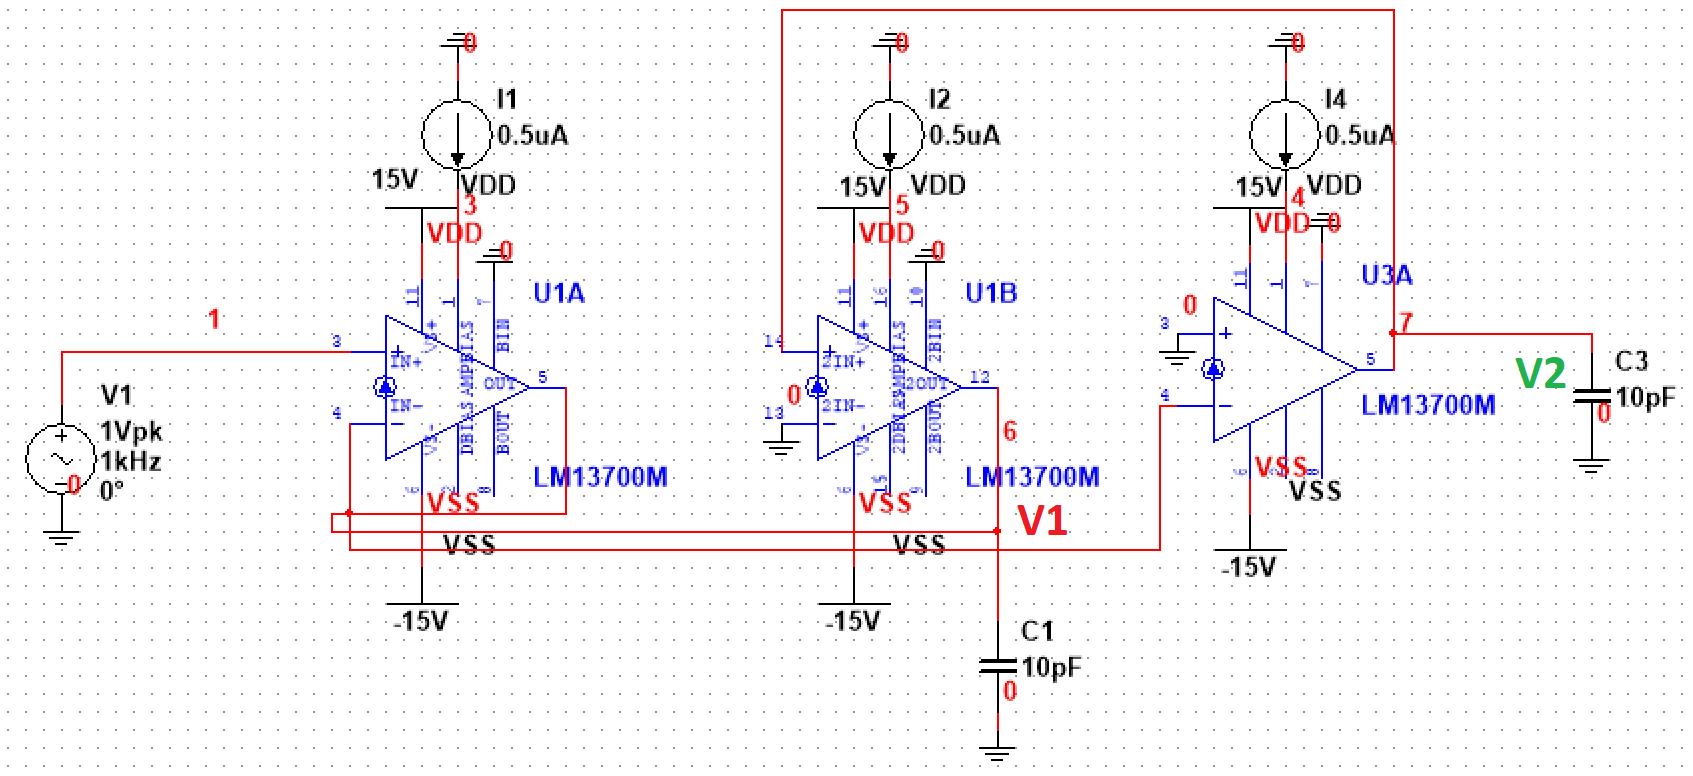
\includegraphics[scale=0.4]{bplp.png}
\end{figure}\begin{figure}[H]
\centering
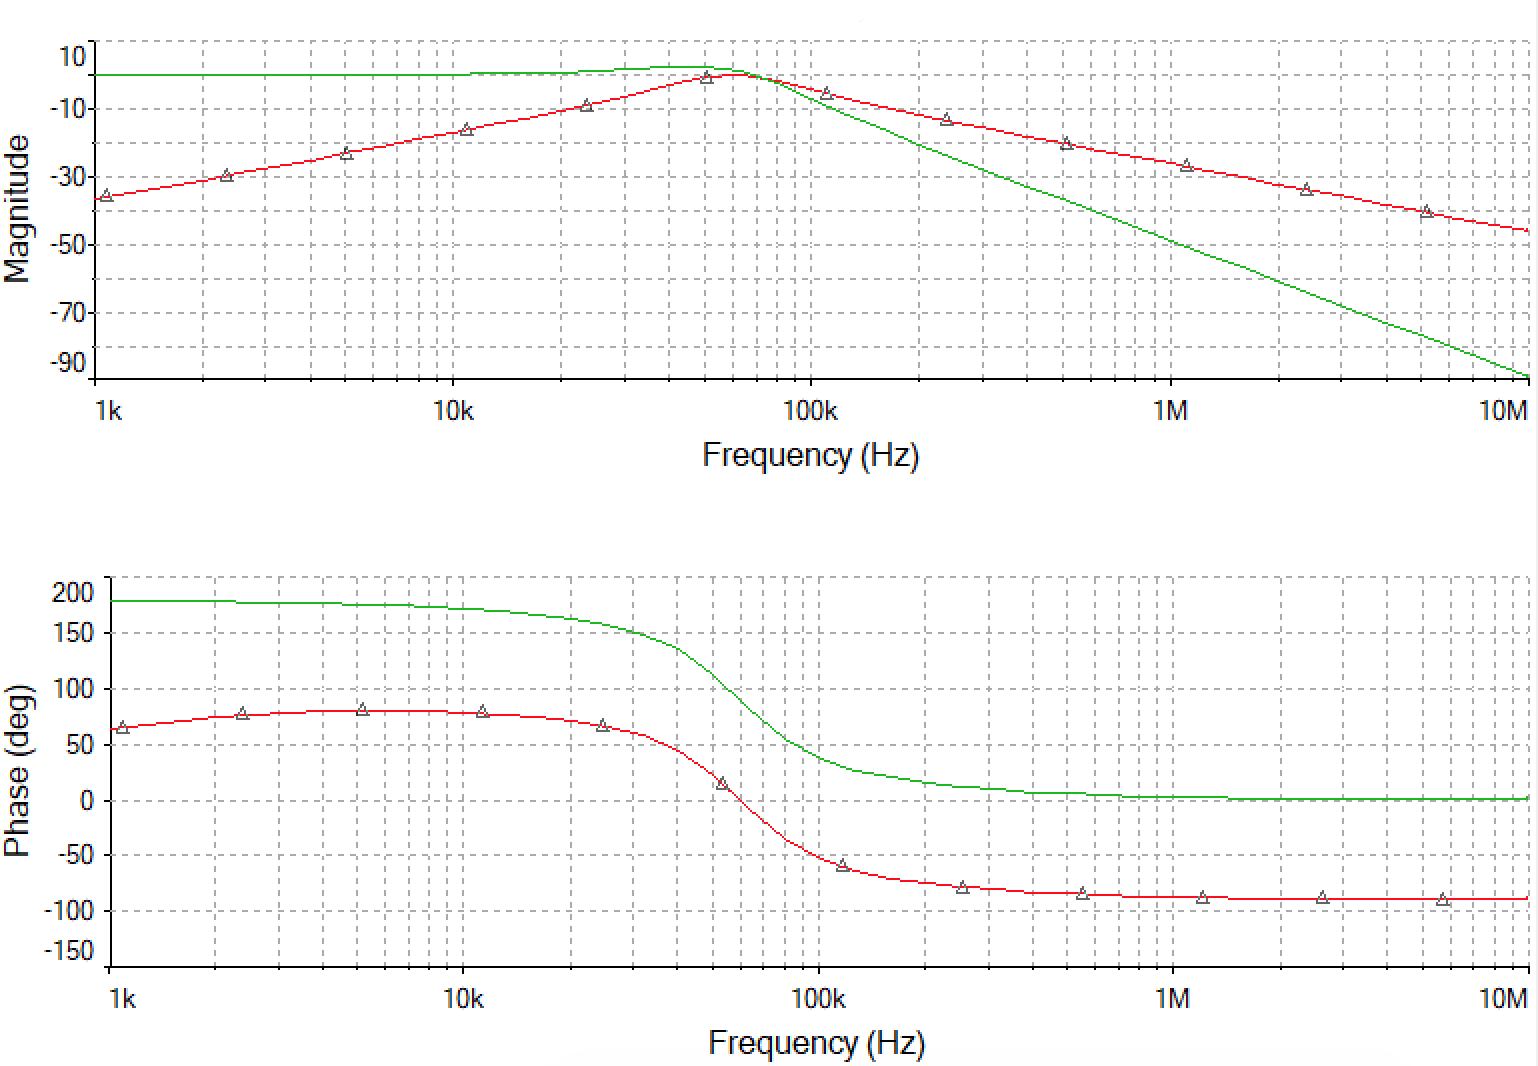
\includegraphics[scale=0.5]{bplp2.png}
\end{figure}
\begin{figure}[H]
\centering
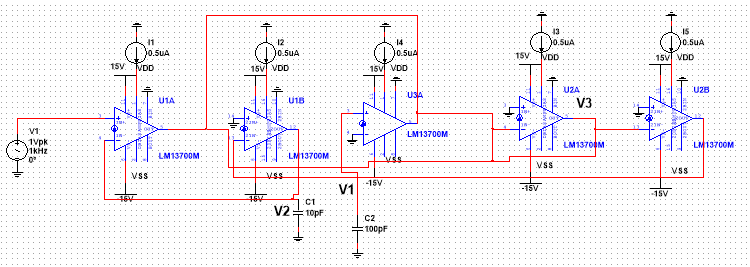
\includegraphics[scale=0.7]{bplphp.png}
\end{figure}
\begin{figure}[H]
\centering
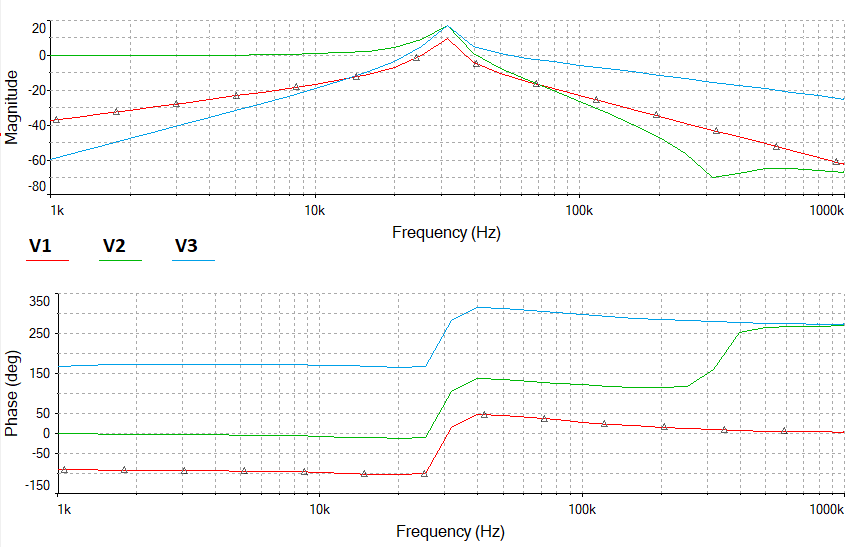
\includegraphics[scale=0.65]{bplphp2.png}
\end{figure}
\begin{figure}[H]
\centering
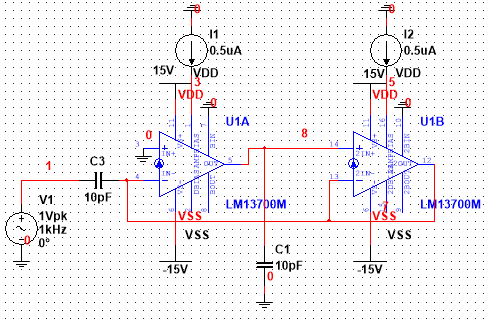
\includegraphics[scale=0.7]{pp2.png}
\end{figure}
\begin{figure}[H]
\centering
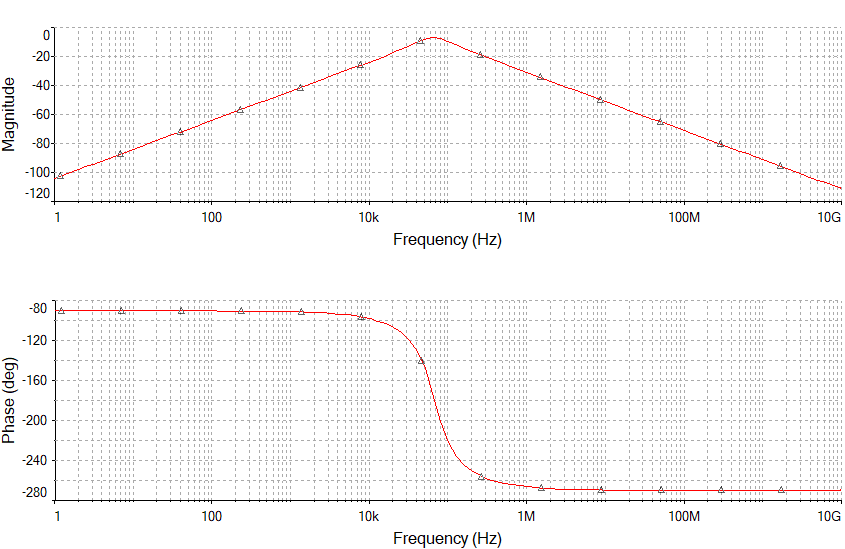
\includegraphics[scale=0.65]{pp.png}
\end{figure}
\end{document}